\begin{flushleft}
{\Huge Punschvisor\\}
\vspace{1cm}
\Large{
Punsch drickes antingen mycket kall till efterrätt alla dagar i veckan,
eller varm till torsdagens ärtsoppa. Det kan även hända att det
slinker ner en liten en till onsdags-hofflan. En gång i tiden hade
punschen systemets högsta apk - Alkohol per Krona - och många tror att
det är därför det alltid har druckits mycket punsch i studentikosa
sammanhang. Andra tror det beror på att det är gott.}
\end{flushleft}
\vspace{2cm}
\begin{center}
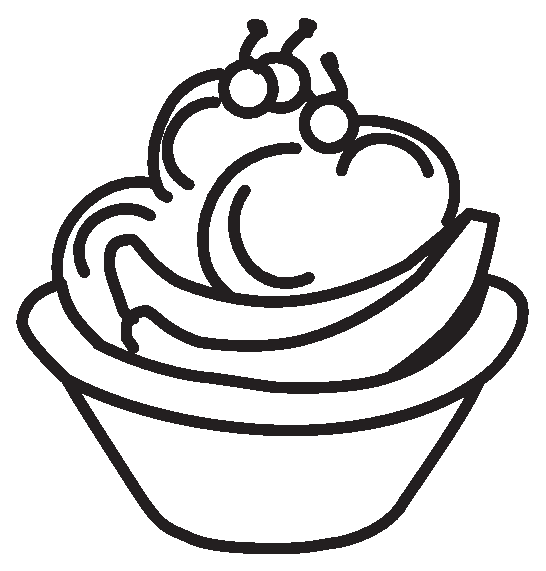
\includegraphics[width=5cm]{bilder/47.eps}
\end{center}
\newpage

\begin{song}{Gamla punschvisan (kall)}{gamlakall}
\mel{Änkevalsen}
\begin{vers}
Punschen kommer, punschen kommer,\\
ljuv och sval.\\
Glasen imma, röster stimma,\\
i vår sal.\\
Skål för glada minnen!\\
Skål för varje vår!\\
Inga sorger finnas mer,\\
när punsch vi får!\\
\end{vers}
\end{song}

\begin{song}{Gamla punschvisan (varm)}{gamlavarm}
\mel{Änkevalsen}
\begin{vers}
Punschen kommer, punschen kommer,\\
god och varm.\\
Vettet svinner, droppen rinner,\\
ner i tarm.\\
Skål för alla minnen!\\
dem vi snart ej ha,\\
då ett par glas simmig punsch \\
vi hunnit ta!\\
\end{vers}
\end{song}

\newpage

\begin{song}{Punschvisa F}{punschvisaf}
	\mel{Fritiof och Carmencita}
	\begin{vers}
		Cederlunds torr eller Platins vi har i glasen\\
		det är det bästa som vi får här på kalasen.\\
		Glöm morgondagen, låt det skvalpa i magen\\
		för med punsch uti glasen dricka vi till Dragos lov\\
		Huka dig Bacchus, nu, ty punschen den är sval\\
		Ah! Det gör så gott ååt strupen.
	\end{vers}
	\begin{vers}
		Carlshamns flaggpunsch och Grönstedts blå\\
		det är en blandning som förunnad är åt få \\
		Men på bordet bredvid koppen, med en yta så klar\\
		där står punschen och väntar på att drickas.\\
		Nu är det dags för bacchanal\\
		Glöm bort fysiken med dess fruktansvärda kval\\
		för nu höjer vi upp glasen, ropar ut en samfälld SKÅL!\\
	\end{vers}
	\begin{vers}
		(Klunk)
	\end{vers}
	\begin{vers}
		Ah! Det gjorde gott ååt strupen.
	\end{vers}
\end{song}

\newpage


\begin{song}{Festu:s punschvisa}{festu}
\mel{Tomtarnas julnatt}
\begin{vers}
Punschen, punschen rinner genom strupen,\\
ner i djupen.\\
Blandas, konfronteras där med supen,\\
där med supen.\\
Gula droppar stärker våra kroppar.\\
PUNSCH, PUNSCH, PUNSCH\\
\end{vers}
\end{song}

\begin{song}{Studiemedelsrondo}{studiemedelsrondo}
\mel{Ösa sand}
\begin{vers}
//:Vi dricker punsch\\
till lunch\\
när vi har fått avin.\\
Vi lunchar hela dagen\\
tills kassan gått i sin.://\\
\end{vers}
\end{song}

\newpage

\begin{song}{Punschen gul}{punschengul}
\mel{Vem kan segla}
\begin{vers}
Punschen gul uppå bordet står.\\
Punschen snällt på dig vänta.\\
Om din längtan till punschen går,\\
ta den utan att flämta.\\
\end{vers}
\end{song}

\begin{song}{Djungelpunsch}{djungelpunsch}
\mel{Var nöjd med allt som livet ger}
\begin{vers}
Jag gillar alla tiders punsch,\\
en punsch till frukost, punsch till lunch,\\
en punsch till förrätt, varmrätt och dessert.\\
Jag gillar punsch för vet du vad -\\
rent kaffe gör ju ingen glad.\\
Så punsch i fulla muggar vill jag ha!\\
\end{vers}
\end{song}

\newpage

\begin{song}{En kopp med punsch}{enkoppmedpunsch}
\mel{Med en enkel tulipan}
\begin{vers}
Nu med en ny och stadig krök\\
med armen gör vi försök\\
att lyfta koppen, att lyfta koppen\\
som står och väntar.\\
Håll blicken fäst vid koppens rand\\
och darra inte på hand.\\
Nu allesammans, nu allesammans\\
på munnen gläntar.\\
\end{vers}
\begin{vers}
En liten punschtår så här placerad\\
i ena handen sig bättre gör\\
än tio liter på systemet\\
och inga pengar att köpa för.\\
\end{vers}
\begin{vers}
Spill inga droppar på ditt bord\\
och spill ej mer några ord.\\
Nu tar vi punschen, nu tar vi punschen\\
som står och väntar.\\
\end{vers}
\end{song}

\newpage

\begin{song}{Gudarnas punschvisa}{gudarnaspunschvisa}
\mel{Sov du lilla videung}
\begin{vers}
Snart vi tömmer våran punsch\\
med en knyck på armen.\\
Punsch till frukost, punsch till lunch,\\
det är mums för tarmen!\\
Nästan hela dagarna\\
är det gott i magarna.\\
Luta dig mot karmen,\\
njut i hela barmen!\\
\end{vers}
\end{song}

\begin{song}{Punschschottis}{punschschottis}
\mel{Schottis på Valhall}
\begin{vers}
Uppå bordet står nu en liten tår,\\
den har lyster precis som kristall.\\
Den är lockande, den är pockande,\\
och fast den är isande kall,\\
Den oss värme ger när den slunkit ner\\
i en dammig och torr liten hals.\\
Det är punschen som går,\\
det är punschen som får\\
hela livet att bli till en vals.\\
\end{vers}
\end{song}

\newpage

\begin{song}{Änglapunsch}{anglapunsch}
\mel{Änglamark}
\begin{vers}
Kalla den gudagåva eller himlanektar, vad du vill;\\
punschen den gyll'ne, de gamla oss skänkte.\\
Vet att så länge som punschen nånsin funnits till\\
glädjen den höjde och sorgerna dränkte.\\
\end{vers}
\begin{vers}
Blunda och dröm om en blommande sommarnatt\\
svala bersåer där punschen står immig.\\
Eller en höstdag när Nordan har lekt tafatt\\
varm punsch som ångar och ärtsoppa simmig.\\
\end{vers}
\begin{vers}
Punschen den älskas av alla och envar.\\
Låt festen börja - låt punschen få flöda!\\
Skål alla vänner som har nå't i glaset kvar,\\
hedra nu minnet av gamle kung Oscars da'r!\\
\end{vers}
\begin{vers}
Kalla den gudagåva eller himlanektar, vad du vill;\\
punschen den gyll'ne, som får oss att drömma.\\
Fukta din strupe, låt inte flaskan få stå still.\\
Skåla för punschen och glasen vi tömma!\\
\end{vers}
\end{song}

\newpage

\begin{song}{Punsch-lunch}{punschlunch}
\mel{Jag vill ha blommig falukorv}
\begin{vers}
Jag vill ha kall och simmig punsch till lunch,\\
mamma, nå't annat vill jag inte ha.\\
Øhl får man för ofta, vin smakar som kofta,\\
starksprit det är riktigt läbbigt.\\
Nej, jag vill ha kall och simmig punsch till lunch,\\
mamma, ett stort glas härlig punsch till lunch.\\
\end{vers}
\end{song}

\begin{song}{Skogshögskolans punschvisa}{skogshogskolanspunschvisa}
\textit{Ur Skogshögskolans sångbok 1906}
\begin{vers}
Länge har jag tänkt \\
att punschen övergiva.\\
Men det får ej ske,\\
så länge jag får leva.\\
För när jag en gång dör\\
så står det på min grav:\\
Här vilar en som svenska \\
punschen älskat har.\\
\end{vers}
\end{song}

\begin{song}{Jag gillar}{jaggillar}
\begin{vers}
Jag gillar, jag gillar punschen.\\
Jag gillar den som punschen skapat har.\\
Jag gillar, jag gillar punschen.\\
Jag gillar punschen och dess far!\\
\end{vers}
\begin{vers}
Jag gillar, jag gillar punken.\\
Jag gillar den som punken skapat har.\\
Sex Pistols och Magnus Uggla.\\
De är så j-a, j-a bra! 
\end{vers}
\end{song}

\newpage

\begin{song}{Ärter och punsch}{arterochpunsch}
\mel{Fritiof och Carmencita}
\begin{vers}
Ärter och punsch en liten rätt med traditioner,\\
den smakar bra och väcker många sensationer,\\
blekgul till färgen, smaken går intill märgen,\\
med en senap som blandas enligt gammal tradition.\\
Så skall den njutas denna svenska folkspassion\\
en torsdagskväll i varje månad.\\
\end{vers}
\begin{vers}
Skål vänner, bort med all tristess,\\
ärter och punsch det ska vi njuta utan stress,\\
inga sura miner vill vi se i afton,\\
när doften utav ärter och punsch sprids i salongen.\\
Tänk på Grönstedt, Cederlund och Flagg,\\
åh - vilken doft från denna arraksgula tagg.\\
Hela natten ska vi njuta denna underbara brygd\\
skål för lilla ärtan och punschen.\\
\end{vers}
\end{song}

%\begin{song}{När som punschen}{narsompunschen}
%\mel{Barndomshemmet}
%\begin{vers}
%När som punschen rinner nedför strupen,\\
%står min mage där och kastar upp igen.\\
%\end{vers}
%\end{song}

\newpage
\begin{song}{Tvekan inför punschen}{tvekaniforpunschen}
\mel{Rosa på bal\\text: Håkan 'Sebbe' Jakobsson}
\begin{vers}
Jag borde nog inte dricka mer,\\
varken øhl eller vin eller brännevin.\\
En kaffetår blott, men så vitt jag ser \\
Står en punsch brevi'n.\\
\end{vers}
\begin{vers}
Tänk vilken underbar färg och odör!\\
-Nej, det blir bara man bråkar och stör.\\
Men för att inte min kväll ska bli trist,\\
krävs både slughet och list.\\
\end{vers}
\begin{vers}
Så jag tror nog att jag tar en\\
punsch, kanske två, kanske tre!\\
Se'n blir det groggar i baren,\\
jag klarar säkert av det.
\end{vers}
\begin{vers}
Trots att egentligen jag är rätt knall,\\
piggar nog punsch upp mig i alla fall.\\
Jag kvicknar till med en punsch i min bål.\\
Nu har jag bestämt mig, SKÅL!\\
\end{vers}
\end{song}

\newpage

\begin{song}{Punschpolkett}{punschpolkett}
\mel{Nudistpolka}
\begin{vers}
Inte dricker jag snaps\\
nej, det passar ej alls\\
till en kaffetår en kväll, \\
men av punschen blir man säll\\
för se punschen går idag som igår.\\
Går till ärter och glass,\\ 
är en dryck utav klass,\\
har en söt och välkänd smak.\\
Oh, vad det är underbart\\
att få tömma punschpokalen!\\
HOPPSANSA!\\
\end{vers}
\end{song}

\begin{song}{Min punsch}{minpunsch}
\mel{Min häst}
\begin{vers}
//:Min punsch den är söt och ljusgul.\\
Jag dricker den varm som kall.\\
Till mina ärtor med fläsk\\
och efter en Bäsk\\
när punschen smakar som bäst i magen://\\
\end{vers}
\end{song}

\newpage

\begin{song}{Punsch, punsch}{punschpunsch}
\mel{Bä, bä, vita lamm}
\begin{vers}
Punsch, punsch, lilla vän,\\
dricker vi ikväll.\\
Punsch, punsch får du sen,\\
så att du blir säll.\\
Cederlunds till far,\\
och Carlshamns Flagg åt mor,\\
och hemgjord blandning\\
åt lille, lille bror\\
\end{vers}
\end{song}

\begin{song}{Punch, punch}{punchpunch}
\mel{Ritsch, ratsch}
\begin{vers}
Punch punch filibombombom,\\
filibombombom, filibombombom\\
Punch punch filibombombom,\\
filibombombom, filibom\\
\end{vers}
\begin{vers}
Vi har ju både Cederlunds och Carlshamns flagg\\
och Grönstedts blå och lilla Caloric.\\
Det blir för trist med sodavatten,\\
sodavatten, sodavatten\\
Det blir för trist med sodavatten,\\
nej, ge mig lite punch\\
\end{vers}
\end{song}

\newpage

\begin{song}{Vädjan till punschen}{vadjantillpunschen}
\mel{Sov du lilla videung}
\begin{vers}
Kom nu lilla punschen min\\
följ nu efter supen.\\
Snart så skall du åka in\\
ner igenom strupen.\\
Till mitt stora magpalats,\\
där det finns så mycket plats.\\
Kom nu lilla punschen \\
följ nu efter supen.\\
\end{vers}
\end{song}

\begin{song}{Sista punschvisan}{sistapunschvisan}
\mel{Auld lang syne}
\begin{vers}
När punschen småningom är slut\\
och vår flaska blivit tom,\\
då vänder vi den upp och ner\\
till dess inget rinner ur.\\
\end{vers}
\begin{vers}
//: Så slickar vi, så slickar vi\\
båd' utanpå och i\\
och finns det ändå något kvar\\
får det va till sämre dar. ://\\
\end{vers}
\end{song}






